%%%%%%%%%%%%%%%%%%%%%%%%%%%%%%%%%%%%%%%%%
% University/School Laboratory Report
% LaTeX Template
% Version 3.1 (25/3/14)
%
% This template has been downloaded from:
% http://www.LaTeXTemplates.com
%
% Original author:
% Linux and Unix Users Group at Virginia Tech Wiki 
% (https://vtluug.org/wiki/Example_LaTeX_chem_lab_report)
%
% License:
% CC BY-NC-SA 3.0 (http://creativecommons.org/licenses/by-nc-sa/3.0/)
%
%%%%%%%%%%%%%%%%%%%%%%%%%%%%%%%%%%%%%%%%%

%----------------------------------------------------------------------------------------
%	PACKAGES AND DOCUMENT CONFIGURATIONS
%----------------------------------------------------------------------------------------

\documentclass{article}

\usepackage{polski}
\usepackage[utf8]{inputenc}
\usepackage{booktabs}
\usepackage{multirow}
\usepackage{caption}

\usepackage[version=3]{mhchem} % Package for chemical equation typesetting
\usepackage{siunitx} % Provides the \SI{}{} and \si{} command for typesetting SI units
\usepackage{graphicx} % Required for the inclusion of images
\usepackage{natbib} % Required to change bibliography style to APA
\usepackage{amsmath} % Required for some math elements 

\setlength\parindent{0pt} % Removes all indentation from paragraphs

\renewcommand{\labelenumi}{\alph{enumi}.} % Make numbering in the enumerate environment by letter rather than number (e.g. section 6)
\usepackage{color}

%\usepackage{times} % Uncomment to use the Times New Roman font

%----------------------------------------------------------------------------------------
%	DOCUMENT INFORMATION
%----------------------------------------------------------------------------------------

\title{Ćwiczenie nr 41: Busola stycznych} % Title

\author{Rafał \textsc{Grabiański} i Zbigniew \textsc{Królikowski}} % Author name

\date{\today} % Date for the report

\addtolength{\oddsidemargin}{-.875in}
\addtolength{\evensidemargin}{-.875in}
\addtolength{\textwidth}{1.75in}
\addtolength{\topmargin}{-.875in}
\addtolength{\textheight}{1.75in}

\begin{document}

% Please add the following required packages to your document preamble:
% \usepackage{booktabs}
\begin{table}[h]
\begin{tabular}{@{}llllll@{}}
\toprule
\begin{tabular}[c]{@{}l@{}}Wydział:\\ \\ WIEiT\end{tabular}                                    & \multicolumn{2}{l}{\begin{tabular}[c]{@{}l@{}}Imię i nazwisko:\\ Rafał Grabiański\\ Zbigniew Królikowski\end{tabular}}                & \begin{tabular}[c]{@{}l@{}}Rok:\\ \\ II\end{tabular}            & \begin{tabular}[c]{@{}l@{}}Grupa:\\ \\ 7\end{tabular}              & \begin{tabular}[c]{@{}l@{}}Zespół:\\ \\ 7\end{tabular} \\ \midrule
\multicolumn{1}{|c|}{\begin{tabular}[c]{@{}c@{}}PRACOWNIA\\ FIZYCZNA\\ WFiIS AGH\end{tabular}} & \multicolumn{4}{l|}{Temat: Kriogenika}                                                                                                                                                                                                                                                  & \multicolumn{1}{l|}{Nr ćwiczenia: 113}                     \\ \midrule
\begin{tabular}[c]{@{}l@{}}Data wykonania:\\ \\ \\ 16.12.2014\end{tabular}                     & \begin{tabular}[c]{@{}l@{}}Data oddania:\\ \\ \\ 13.01.2015\end{tabular} & \begin{tabular}[c]{@{}l@{}}Zwrot do poprawy:\\ \\ \\ .\end{tabular} & \begin{tabular}[c]{@{}l@{}}Data oddania:\\ \\ \\ .\end{tabular} & \begin{tabular}[c]{@{}l@{}}Data zaliczenia:\\ \\ \\ .\end{tabular} & OCENA:                                                  \\ \bottomrule
\end{tabular}
\end{table}

%\maketitle % Insert the title, author and date

% If you wish to include an abstract, uncomment the lines below


%----------------------------------------------------------------------------------------
%	SECTION 1 - CEL ĆWICZENIA
%----------------------------------------------------------------------------------------

\section{Cel ćwiczenia}

Celem ćwiczenia było zapoznanie się z budową i działaniem przyrządu nazwanego busolą stycznych. Mieliśmy za zadanie wyznaczyć doświadczalnie składową poziomą ziemskiego pola magnetycznego.

% If you have more than one objective, uncomment the below:
%\begin{description}
%\item[First Objective] \hfill \\
%Objective 1 text
%\item[Second Objective] \hfill \\
%Objective 2 text
%\end{description}

 

%\clearpage

%----------------------------------------------------------------------------------------
%	SECTION 4
%----------------------------------------------------------------------------------------
\section{Wyniki pomiarów}
\begin{table}[htbp]
\centering
\scalebox{0.65}{
\begin{tabular}{|c|r|r|r|r|r|r|}
\hline
Lp & \multicolumn{1}{c|}{Liczba Zwojów n} & \multicolumn{1}{c|}{Prąd [mA]} & \multicolumn{1}{c|}{Kąt w lewo [$^o$]} & \multicolumn{1}{c|}{Kąt w prawo [$^o$]} & \multicolumn{1}{c|}{Średni kąt [$^o$]} & \multicolumn{1}{c|}{B [$\mu T$]} \\ \hline
1 & 12 & 300 & 35 & 35 & 35 & 2.48 \\ \hline
2 & 12 & 350 & 40 & 40 & 40 & 2.42 \\ \hline
3 & 12 & 250 & 29 & 31 & 30 & 2.51 \\ \hline
4 & 12 & 200 & 26 & 24 & 25 & 2.49 \\ \hline
5 & 16 & 200 & 32 & 32 & 32 & 2.48 \\ \hline
6 & 16 & 250 & 38 & 38 & 38 & 2.47 \\ \hline
7 & 16 & 150 & 26 & 25 & 25.5 & 2.43 \\ \hline
8 & 16 & 180 & 30 & 29 & 29.5 & 2.46 \\ \hline
9 & 24 & 100 & 27 & 27 & 27 & 2.28 \\ \hline
10 & 24 & 150 & 34 & 36 & 35 & 2.48 \\ \hline
11 & 24 & 180 & 39 & 40 & 39.5 & 2.53 \\ \hline
12 & 24 & 130 & 32 & 32 & 32 & 2.41 \\ \hline
13 & 36 & 50 & 21 & 20 & 20.5 & 2.33 \\ \hline
14 & 36 & 100 & 35 & 36 & 35.5 & 2.44 \\ \hline
15 & 36 & 120 & 40 & 40 & 40 & 2.49 \\ \hline
16 & 36 & 80 & 28 & 30 & 29 & 2.51\\ \hline
17 & 40 & 50 & 22 & 22 & 22 & 2.39\\ \hline
18 & 40 & 70 & 29 & 29 & 29 & 2.44 \\ \hline
19 & 40 & 90 & 34 & 34 & 34 & 2.58 \\ \hline
20 & 40 & 110 & 41 & 41 & 41 & 2.45 \\ \hline
\end{tabular}
}
\caption{Wyniki pomiarów dla różnych wartości prądu płynącego w zwojnicy}
\label{}
\end{table}

\begin{figure}[h!]
\centering
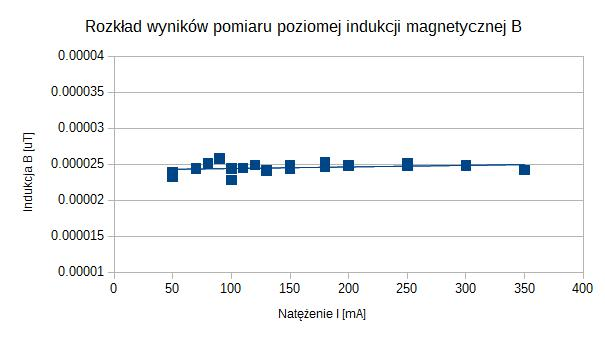
\includegraphics[scale=0.53]{ch01}
\end{figure}


%----------------------------------------------------------------------------------------
%	SECTION 5 - WYNIKI
%----------------------------------------------------------------------------------------

\section{Opracowanie wyników}
\subsection{Obliczenie wartości poziomej składowej indukcji ziemskiego pola magnetycznego}

Wartość poziomej indukcji magnetycznej wyliczyliśmy z zależności:
\begin{equation}
B_0 = \mu_0 \cdot \frac{NI}{2R \, tg \alpha}
\end{equation}

Wartość średnią poziomej indukcji magnetycznej obliczyliśmy licząć średnią arytmetyczną ze wszystkich pomiarów.
$B_0 = \overline{B} = (2.45 \pm 0.28) \cdot 10^{-5} \mu T$
\newline
\subsection{Obliczenie niepewności pomiarowych}
Niepewność wyliczonej indukcji policzyliśmy z odchylenia standardowego średniej uzyskanych pomiarów.
\begin{equation}
u_A(B_0) = 6.8 \cdot 10^{-7} \mu T
\end{equation}
Czyli względna niepewność:
\begin{equation}
\frac{u_A(B_0)}{B_0} \approx 2.8\%
\end{equation}

Niepewności typu B będą dotyczyły amperomierza:
\begin{equation}
\Delta I = \frac{zakres \, x \, klasa}{100} = 56 mA
\end{equation}

\begin{equation}
u_B(I) = \frac{\Delta I}{\sqrt{3}} = 32.3 mA 
\end{equation}

\begin{equation}
\frac{u_B(I)}{I} = 11 \%
\end{equation}

Niepewność pomiaru grubości cewki oszacowaliśmy grubo przyjmując, z racji odczuwalnych różnic w geometrii i rozdzielczości miary na 3 mm.
Względny błąd wyniesie zatem:
\begin{equation}
\frac{u_B(R)}{R} = 	\frac{3}{130} \approx 2.3 \%
\end{equation}
Na koniec obliczamy względną niepewność złożoną: \\ \newline
\newline
\centerline{$\frac{u_c(B_0)}{B_0} = \sqrt{[\frac{u_A(B_0)}{B_0}]^2 + [\frac{u_B(I)}{I}]^2 + [\frac{u_B(R)}{R}]^2} = \sqrt{[2.8\%]^2+[11\%]^2+[2.3\%]^2} \approx 11.6 \%$}
\newline
\newline
I z tego liczymy $u_c(B_0) = 2.84 \cdot 10^{-6} \mu T$


\newpage

%----------------------------------------------------------------------------------------
%	SECTION 6
%----------------------------------------------------------------------------------------
\section{Wnioski}

Otrzymana wartość składowej poziomej natężenia pola magnetycznego Ziemi dla Krakowa, wyniosła $B_0 = (2.45 \pm 0.28) \cdot 10^{-5} \mu T$. W porównaniu do wartości tabelarycznej: $B_T = 2.1 \cdot 10^{-5} \mu T$ oraz k=2 mieścimy się przedziale w niepewności rozszerzonej ($1.53 \cdot 10^{-5} \mu T$, $2.67 \cdot 10^{-5} \mu T$).

Nie używając niepewności rozszerzonej wykroczyliśmy tylko nieznacznie poza przedział, co świadczy o prawidłowym wykonaniu doświadczenia. Nie zaobserwowano błędów grubych.

Największy wpływ na niepewność pomiaru miała mała rozdzielczość amperomierza równa $u_c 2.8 mA T$, a największa możliwa do otrzymania niepewność wyniosła: \begin{equation}
\Delta I = \frac{zakres \, x \, klasa}{100} = 56 mA
\end{equation}

%----------------------------------------------------------------------------------------
%	BIBLIOGRAPHY
%----------------------------------------------------------------------------------------

\bibliographystyle{apalike}

\bibliography{sample}
%----------------------------------------------------------------------------------------


\end{document}
